% Copyright © 2012, 2014 Martin Ueding <dev@martin-ueding.de>
%
\documentclass[11pt, ngerman, fleqn]{article}

\usepackage[a4paper, left=3cm, right=2cm, top=2cm, bottom=2cm]{geometry}
\usepackage[activate]{pdfcprot}
\usepackage[thinspace, squaren]{SIunits}
\usepackage[iso]{isodate}
\usepackage[parfill]{parskip}
\usepackage[T1]{fontenc}
\usepackage[utf8]{inputenc}
\usepackage{amsmath}
\usepackage{amsthm}
\usepackage{babel}
\usepackage{color}
\usepackage{lastpage}
\usepackage{commath}
\usepackage{epstopdf}
\usepackage{fancyhdr}
\usepackage{graphicx}
\usepackage{hyperref}
\usepackage{setspace}
\usepackage{tikz}

\usepackage[charter, greekuppercase=italicized]{mathdesign}

\usetikzlibrary{arrows}
\usetikzlibrary{intersections}

\definecolor{darkblue}{rgb}{0,0,.5}
\definecolor{darkgreen}{rgb}{0,.5,0}

\hypersetup{
	breaklinks=false,
	citecolor=darkgreen,
	colorlinks=true,
	linkcolor=black,
	menucolor=black,
	urlcolor=darkblue,
}

\setlength{\columnsep}{1.5cm}

\DeclareMathOperator{\arcsinh}{arsinh}
\DeclareMathOperator{\arsinh}{arsinh}
\DeclareMathOperator{\asinh}{arsinh}
\DeclareMathOperator{\card}{card}
\DeclareMathOperator{\diam}{diam}

\newcommand{\dalambert}{\mathop{{}\Box}\nolimits}
\newcommand{\divergence}[1]{\inner{\vnabla}{#1}}
\newcommand{\ee}{\mathrm e}
\newcommand{\emesswert}{\del{\messwert \pm \messwert}}
\newcommand{\e}[1]{\cdot 10^{#1}}
\newcommand{\fehlt}{\textcolor{red}{Hier fehlen noch Inhalte.}}
\newcommand{\half}{\frac 12}
\newcommand{\ii}{\mathrm i}
\newcommand{\inner}[2]{\left\langle #1, #2 \right\rangle}
\newcommand{\laplace}{\mathop{{}\bigtriangleup}\nolimits}
\newcommand{\messwert}{\textcolor{blue}{\square}}
\newcommand{\punkte}{\textcolor{white}{xxxxxxx}}
\newcommand{\tens}[1]{\boldsymbol{\mathsf{#1}}}
\newcommand{\vnabla}{\vec \nabla}
\renewcommand{\vec}[1]{\boldsymbol{#1}}

\newcommand{\themodul}{physik311}
\newcommand{\thegruppe}{Gruppe 3 -- Matthias Rehberger}
\newcommand{\theuebung}{7}

\pagestyle{fancy}

\fancyfoot[C]{\footnotesize{\thegruppe}}
\fancyfoot[L]{\footnotesize{Martin Ueding}}
\fancyfoot[R]{\footnotesize{Seite \thepage\ / \pageref{LastPage}}}
\fancyhead[L]{\themodul{} -- Übung \theuebung}

\setcounter{section}{23}

\def\thesubsection{\thesection\alph{subsection}}

\title{\themodul{} -- Übung \theuebung \\ \vspace{0.5cm} \large{\thegruppe}}

\author{Martin Ueding \\ \small{\href{mailto:mu@uni-bonn.de}{mu@uni-bonn.de}}}

\begin{document}

\maketitle

\begin{table}[h]
	\centering
	\begin{tabular}{l|c|c|c|c}
		Aufgabe & \ref{1} & \ref{2} & \ref{3} & $\sum$   \\
		\hline
		Punkte & \punkte & \punkte & \punkte & \punkte
	\end{tabular}
\end{table}

%%%%%%%%%%%%%%%%%%%%%%%%%%%%%%%%%%%%%%%%%%%%%%%%%%%%%%%%%%%%%%%%%%%%%%%%%%%%%%%
%                             Projektionsapparat                              %
%%%%%%%%%%%%%%%%%%%%%%%%%%%%%%%%%%%%%%%%%%%%%%%%%%%%%%%%%%%%%%%%%%%%%%%%%%%%%%%

\section{Projektionsapparat}
\label 1

\subsection{Entfernung}

Die Entfernung lässt sich durch die Abbildungsgleichung geben:
\[
	\frac 1g + \frac 1b = \frac 1f
\]

Ich erhalte:
\[
	g = \unit{1.02}{\deci\meter}
\]

\subsection{Abbildungsfehler}

Anscheinend soll das Objektiv möglichst fehlerfrei sein, da es ansonsten zu
Farbfehlern und Unschärfe kommen kann. Wenn es im Kondensor allerdings schon zu
chromatischer Aberration kommt, würde auch ein fehlerfreies Objektiv daran
nichts mehr ändern können. Wahrscheinlich muss gerade das Objektiv möglichst
fehlerarm sein, weil wir es hier als eine Linse ansehen möchten.

Außerdem ist das Objektiv nur dazu da, die Ausdehnung der Lichtquelle zu
korrigieren (siehe folgende Aufgaben). Bei einer ausreichend kleinen
Lichtquelle ist das Objektiv zunehmend irrelevant. Womit wieder höhere
Anforderungen an den Kondensor gestellt werden.

\subsection{Abbildung der Lichtquelle}

Da in dieser Aufgabe alle Linsen dünn sind, darf ich die beiden Linsen des
Kondensors zu einer zusammenfassen. Deren Brennweite ist:
\[
	f_K := \del{\frac 1{f_{K_1}} + \frac 1{f_{K_2}}}^{-1}
	= \unit{2.625}{\centi\meter}
\]

Es ist wahrscheinlich am sinnvollsten, wenn der Kondensor die Lichtquelle in
den Mittelpunkt des Objektives abbildet. Bei einer Punktförmigen Lichtquelle
würde das Objektiv dann nichts an den Strahlen ändern. Da die Lichtquelle
allerdings ausgedehnt ist, sorgt das Objektiv dafür, dass alle Strahlen vom
gleichen Punkt des Dias (das direkt nach der zweiten Kondensorlinse anzubringen
ist) auch auf dem Schirm den gleichen Punkt treffen, also ein scharfes Bild
entsteht.

\subsection{Abstand Lichtquelle}

\paragraph{Kondensordurchmesser}

Der Kondensor muss mindestens so groß sein wie das Dia in der Diagonalen groß
ist, also $\unit{5.67}{\centi\meter}$. Darüber hinaus gibt es Strahlen wie den
pinken in Abbildung \ref{241}, der eine großere erste Kondensorlinse
voraussetzt. Allerdings bin ich mir nicht sicher, wie ich dies errechnen kann.

\begin{figure}
	\centering
	%\includegraphics[width=\textwidth]{241.pdf}
	\caption{%
	Grobe Skizze. Von links nach rechts: Lichtquelle im Brennpunkt, $K_1$,
	$K_2$, Bild der Lichtquelle im Brennpunkt von $K_2$, Schirm.
	}
	\label{241}
\end{figure}

\paragraph{Abstände}

Der Abstand zwischen Lichtquelle und Linse $K_1$ sollte gerade $f_{K_1}$ sein,
damit das Licht wie in der Skizze der Aufgabenstellung gezeigt parallel aus der
ersten Linse kommt. Der Abstand zwischen Linse $K_2$ und dem Objektiv sollte
gerade $f_{K_2}$ sein, damit in der Mitte des Objektivs ein reales Bild der
Lichtquelle entstehen kann.

\subsection{Objektivdurchmesser}

Ich nehme hier an, dass der Kondensor als eine Sammellinse zu betrachten ist.
In Abbildung \ref{242} ist eine maßstabsgetreue Skizze von der Konfiguration
gezeigt. Dabei ist die Lampe jetzt nicht mehr im Brennpunkt der einen
Kondensorlinse, weil die Brechkraft höher ist. Dadurch entsteht durch die eine,
kombinierte, Linse auch ein reales Bild in der Endlichkeit. Zur Konstruktion
des Bildes müsste man den Schnittpunkt des gelben mit dem orangen Strahl
konstruieren, allerdings sollte das erst in $\unit 5 \meter$ Entfernung
gelingen.

\begin{figure}
	\centering
	%\includegraphics[width=\textwidth]{242.pdf}
	\caption{%
	Maßstabsgetreue Skizze. Von links nach rechts: Lichtquelle, Brennpunkt
	Kondensor, Kondensor, Brennpunkt Objektiv, Brennpunkt Kondensor, Objektiv,
	Brennpunkt Objektiv. Ein Kästchen in der Breite entspricht
	$\unit{1}{\centi\meter}$, ein Kästchen in der Höhe entspricht
	$\unit{5}{\milli\meter}$.
	}
	\label{242}
\end{figure}

Mit dem roten und blauen Strahl kann das Bild der Lampe konstruiert werden, es
liegt genau im Objektiv. Das Objektiv ist an diese Stelle plaziert. Der
dunkelblaue (geschätzt) und orange (exakt) Strahl zeigt ungefähr an, wo und wie
groß das Bild wird.

Aus der Skizze ist zu erkennen, dass das Bild der Lampe im Objektiv ungefähr
dreimal so groß wird. Das Objektiv sollte also einen Durchmesser von
$\unit{3}{\centi\meter}$ haben. Mit der Abbildungsgleichung kann ich das exakt
bestimmen und erhalte den gleichen Wert:
\[
	\frac B b = \frac G g
	\quad \leadsto \quad
	G = \frac{\unit{0.5}{\centi\meter}}{\unit{3.5}{\centi\meter}} \cdot \unit{10.5}{\centi\meter}
	= \unit{1.5}{\centi\meter}
\]

Das Objektiv sollte also mindestens $\unit{3}{\centi\meter}$ Durchmesser haben.
Wenn es kleiner ist, werden einige Strahlen vom Rand abgeschnitten, das Bild
bekommt mehr Schärfentiefe, allerdings wird es auch dunkler. Ein größeres
Objektiv könnte nur noch mehr Licht einfangen, wenn der Kondensor auch größer
als das Dia ist.

%%%%%%%%%%%%%%%%%%%%%%%%%%%%%%%%%%%%%%%%%%%%%%%%%%%%%%%%%%%%%%%%%%%%%%%%%%%%%%%
%                           Doppelspaltexperimente                            %
%%%%%%%%%%%%%%%%%%%%%%%%%%%%%%%%%%%%%%%%%%%%%%%%%%%%%%%%%%%%%%%%%%%%%%%%%%%%%%%

\section{Doppelspaltexperimente}
\label 2

\subsection{Maße}

Ich nehme an, dass das Licht in ebenen Wellen den ersten Spalt erreicht. Der
erste Spalt wirkt dann als Einzelspalt. Wenn der Spalt mindestens $d =
\unit{5}{\milli\meter}$ groß ist, dann kommt Licht auf den Doppelspalt. Dann
hätte man auch den einzelnen Spalt weglassen können. Wahrscheinlich soll der
Spalt gerade so bemessen sein, dass das Interferenzmaximum beide Spalte in der
zweiten Platte ausleuchtet.

Der Winkel, der ausgeleuchtet werden soll ist:
\[
	\psi = \frac{\unit{2.5}{\milli\meter}}{\unit 2 \meter} = \unit{1.25}{\milli\radian}
\]

Die Maxima des Einzelspalts liegen bei:
\[
	\frac D \lambda \phi = \half + n
\]

In unserem Fall interessiere ich mich für $D$ und forme um:
\[
	D = \half \frac \lambda \psi = \unit{624}{\micro\meter}
\]

Es ist sinnvoll einen Schlitz anstelle von einem Loch zu nehmen, da die
Intensität mit der Distanz nicht so stark abnimmt. Außerdem sollen weitere
Schlitze beleuchtet werden.

Das Licht kommt also irgendwie am Doppelspalt an. Jetzt streut es dort und die
Maxima liegen bei:
\[
	\sin\phi = \frac{m \lambda}{d} = 1.56\e{-4} \cdot m
	, \quad
	m \in \mathbb Z
\]

Das Interferenzmuster wird extrem fein sein, bei einigen Metern Schirmabstand
gerade so mit dem Auge zu erkennen. Aufgrund des gigantischen Spaltabstandes
sind die einzelnen Maxima ungefähr gleich hell. Es sieht also so aus wie in
Abbildung \ref{f1} und \ref{f2} gezeigt.

\begin{figure}
	\centering
	\begin{minipage}{0.45\textwidth}
		\centering
		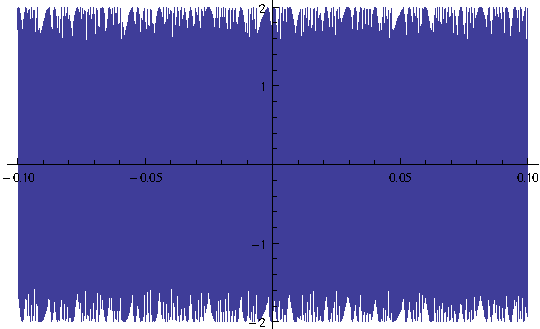
\includegraphics[width=\textwidth]{0,1.pdf}
		\caption{Intensität, für $\phi = \pm \unit{100}{\milli\radian}$}
		\label{f1}
	\end{minipage}
	\hspace{0.08\textwidth}
	\begin{minipage}{0.45\textwidth}
		\centering
		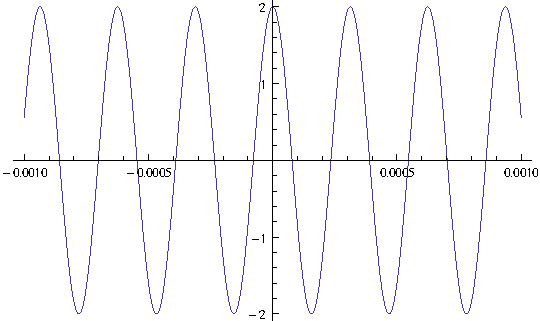
\includegraphics[width=\textwidth]{0,001.pdf}
		\caption{Intensität, für $\phi = \pm \unit{1}{\milli\radian}$}
		\label{f2}
	\end{minipage}
\end{figure}

\subsection{Heliumatome}

Die Rechnungen aus der vorherigen Aufgabe muss ich nur wiederholen. Dabei ist
nun:
\[
	\lambda' = \unit{10.4}{\nano\meter}
	, \quad
	\lambda'' = \unit{10.4}{\micro\meter}
\]

Mit dem neuen Abstand $s' = \unit 1 \meter$ ergibt sich ein neuer Winkel von
$\psi' = \unit{29}{\micro\radian}$ Damit sollte der Eingangsspalt einen
Durchmesser von $D' = \unit{1.79}{\micro\meter}$ beziehungsweise $D'' =
\unit{1.79}{\nano\meter}$ haben.

%%%%%%%%%%%%%%%%%%%%%%%%%%%%%%%%%%%%%%%%%%%%%%%%%%%%%%%%%%%%%%%%%%%%%%%%%%%%%%%
%                                Dipolstrahler                                %
%%%%%%%%%%%%%%%%%%%%%%%%%%%%%%%%%%%%%%%%%%%%%%%%%%%%%%%%%%%%%%%%%%%%%%%%%%%%%%%

\section{Dipolstrahler}
\label 3

Die Frequenz von $f = \unit{30}{\giga\hertz}$ entspricht im Vakuum einer
Wellenlänge von $\lambda = \unit{1}{\centi\meter}$.

In ausreichender Entfernung zur Quelle ist der Gangunterschied von zwei
Strahlen, die dann im Winkel $\phi$ von der Quellenbatterie kommen $\Deltaup s
= \sin\del{\phi} d$ mit $d = \unit{1.5}{\centi\meter}$. Bei diesem
Gangunterschied kommt es zu einer Phasenverschiebung $\delta$, die sich durch
die Wellenlänge ergibt:
\[
	\delta = 2 \pi \sin\del\phi d / \lambda
\]

Die $N = 4$ Wellen, die an einem Punkt zusammenlaufen addiere ich in einem
Phasendiagramm (Abbildung \ref{f3}). Den Radius dieses Kreises kann ich
bestimmen als:
\[
	r = A' \csc\del{\delta/2} / 2
\]

Der halbe Winkel, der sich zwischen den äußersten Schenkeln des großen Dreiecks
bildet, nenne ich $\psi$. Dann kann ich daraus die zusammengesetzte Amplitude
$A$ bestimmen:
\[
	\sin\del\psi = \frac{A/2}{r}
\]

\begin{figure}
	\centering
	\begin{tikzpicture}
		\draw[->] (0, 0) -- ++(0:2) node[below, midway] {$A'$};
		\draw[->] (0, 0) ++(0:2) -- ++(30:2) node[below, midway] {$A'$};
		\draw[->] (0, 0) ++(0:2) ++(30:2) -- ++(60:2) node[right, midway] {$A'$};
		\draw[->] (0, 0) ++(0:2) ++(30:2) ++(60:2) -- ++(90:2) node[right, midway] {$A'$};
		\draw (0, 0) ++(0:2) ++(30:2) ++(60:2) ++(90:2) -- (75:3.8637);
		\draw[thick, <<-] (0, 0) ++(0:2) ++(30:2) ++(60:2) ++(90:2) -- (0, 0) node[midway, below] {$A$};

		\draw (0, 0) -- (75:3.8637) node[left, midway] {$r$};
		\draw (1, 0) -- (75:3.8637);
	\end{tikzpicture}
	\caption{Phasendiagram}
	\label{f3}
\end{figure}

Außerdem ist der ganze Winkel die Summe der Teilwinkel $\delta$, so dass auch
gelten muss:
\[
	2 \psi = \frac{N\delta}{2}
\]

Alles zusammen:
\[
	A = A' \sin\del{\frac{d N \pi}{\lambda} \sin\del\phi} \csc\del{\frac{d \pi}{\lambda} \sin\del\phi}
\]

Maxima entstehen, wenn der der Kosekans gleich 0 wird und der Sinus nicht. Dies
ist bei folgenden Winkeln der Fall:
\[
	\sin\del\phi = m \frac{\lambda}{d}
	\quad\wedge\quad
	\sin\del\phi \neq m \frac{\lambda}{dN}
\]

Also bei
\[
	\sin\del\phi = \frac mN \frac{\lambda}{d}
\]
treten Extremstellen auf, falls $m/N \in \mathbb Z$ liegt, ist es ein Maximum.
Es gibt also mehr Minima als Hauptmaxima.



%\bibliography{../../zentrale_BibTeX/Central}
%\bibliographystyle{plain}

\end{document}

% vim: spell spelllang=de
